% ---------------------------------------------------------------------------------------------------------------
% TEMPLATE PARA TRABALHO DE CONCLUSÃO DE CURSO
% Universidade Federal do Pará
% Modelo da Faculdade de Engenharia Mecânica
% Idealizado por Sérgio Custódio e Kelvin Pinheiro
% Baseado no projeto: http://tcc.tsi.gp.utfpr.edu.br/paginas/modelos-latex-da-utfpr
% De:         Diego Marczal e 
% 	          Michael Vornes 
% ---------------------------------------------------------------------------------------------------------------

% CARREGA CLASSE PERSONALIZADA DA FEM/UFPA--------------------------------------------------------------------------
\documentclass[%twoside,                   % Impressão em frente e verso
oneside,                                   % Impressão apenas frente
]{ufpa-fem-abntex2}

\usepackage{comment}
\usepackage{xcolor}
\usepackage{float}
\usepackage{verbatim}

%INCLUI ARQUIVOS DO TRABALHO DE CONCLUSÃO DE CURSO (PRÉ-TEXTUAIS, TEXTUAIS, PÓS-TEXTUAIS)-----------------------
%%%%%

% INSERE CAPA E FOLHA DE ROSTO
% CAPA-------------------------------------------------------------------

% ORIENTAÇÕES GERAIS-------------------------------------------------------------------------------------
% Caso algum dos campos não se aplique ao seu trabalho, como por exemplo,
% se não houve coorientador, apenas deixe vazio.
% Exemplos: 
% \coorientador{}
% \departamento{}

% DADOS DO TRABALHO--------------------------------------------------------------------------------------
\titulo{\textbf{Um estudo sobre uso de mais de uma licença em projetos de software livres}}
\subtitulo{} %Se não hover subtítulo, deixar em branco.
\titleabstract{Title in English}
\autor{JOÃO PEDRO MOREIRA MORAES}
\autorcitacao{MORAES, João Pedro Moreira} % Sobrenome em maiúsculo
\local{BELÉM/PA}
\data{2019}

% NATUREZA DO TRABALHO-----------------------------------------------------------------------------------
\projeto{Trabalho de Conclusão de Curso}

% TÍTULO ACADÊMICO---------------------------------------------------------------------------------------
\tituloAcademico{Bacharel}

% ÁREA DE CONCENTRAÇÃO E LINHA DE PESQUISA---------------------------------------------------------------
% Se a natureza for Trabalho de Conclusão de Curso, deixe ambos os campos vazios
% Se for programa de Pós-graduação, indique a área de concentração e a linha de pesquisa
\areaconcentracao{}
\linhapesquisa{}

% DADOS DA INSTITUIÇÃO-----------------------------------------------------------------------------------
% Se a natureza for Trabalho de Conclusão de Curso, coloque o nome do curso de graduação em "programa"
% Formato para o logo da Instituição: \logoinstituicao{<escala>}{<caminho/nome do arquivo>}
\instituicao{Universidade Federal do Pará}
\departamento{Instituto de Ciências Exatas e Naturais}
\programa{Ciência da Computação}
\logoinstituicao{2cm}{figuras/naomexafig/logoufpa.png} %

% DADOS DOS ORIENTADORES---------------------------------------------------------------------------------
\orientador{Prof. Dr. Gustavo Henrique Lima Pinto}
%\orientador[Orientadora:]{Nome da orientadora}
\instOrientador{Universidade Federal do Pará}

%\coorientador{Nome do coorientador}
%\coorientador[Coorientadora:]{Nome da coorientadora}
%\instCoorientador{Instituição do coorientador}

% FOLHA DE ROSTO-------------------------------------------------------------------

% Este arquivo não precisa ser alterado

%% TRABALHO DE CONCLUSÃO DE CURSO
\preambulo{{\imprimirprojeto}, apresentado como requisito parcial para a obtenção de grau de {\imprimirtituloAcademico} em Ciência da Computação, pela {\imprimirinstituicao}.}

% ---
% Inserir folha de aprovação
% ---
% Isto é um exemplo de Folha de aprovação, elemento obrigatório da NBR
% 14724/2011 (seção 4.2.1.3). Você pode utilizar este modelo até a aprovação do trabalho. Após isso, substitua todo o conteúdo deste arquivo por uma imagem da página assinada pela banca com o comando abaixo:
%
% \includepdf{folhadeaprovacao_final.pdf}
%


\dataaprovacao{08/03/2019}
\conceito{} %Antes da defesa, não adicionar valor ao compo. Após a defesa, pode-se adicionar Regular, Bom ou Excelente e solicitar as assinaturas da banca examinadora.
 
\nomePrimeiromembro{Richard Matthew Stallman}
\instPrimeiromembro{Instituto de Tecnologia de Massachusetts}
 
\nomeSegundomembro{Ms. Linus Benedict Torvalds}
\instSegundomembro{Universidade de Helsínquia}

%Ocultar ou não dependendo do numero de professores na banca. Ver arquivo de configuracao \assinatura{\imprimirnomeTerceiromembro  \\ Membro - \imprimirinstTerceiromembro}  nas configuracoes ufpa-fem-abntex2.cls.

%\nomeTerceiromembro{Eng. Beltrano Cunha} 
%\instTerceiromembro{Externo (PETROBRAS)}

%ª
 


\newcommand{\gnote}[1]{{\color{red} [#1] - Gustavo}}

\begin{document}
	
	\pretextual
	\imprimircapa                                  \imprimirfolhaderosto{}                           \imprimirfolhadeaprovacao{}                       % DEDICATÓRIA------------------------------------------------------------------

\renewcommand{\dedicatorianame}{DEDICATÓRIA}

\begin{dedicatoria}

Dedico aos meus amados pais.

\end{dedicatoria}
          			% AGRADECIMENTOS---------------------------------------------------------------

\begin{agradecimentos}[AGRADECIMENTOS]

É chegado ao fim um ciclo de muitas risadas, choro, felicidade e frustrações. Sendo assim, dedico este trabalho a todos que fizeram parte desta etapa da minha vida. Agradeço a Deus por ter iluminado o meu caminho, aos meus pais Maria do Socorro Moraes e José Amaral Moraes por terem propiciado a realização deste sonho. E aos amigos que cultivei nessa árdua caminhada.

\end{agradecimentos}

	% EPÍGRAFE---------------------------------------------------------------------

\renewcommand{\epigraphname}{EPÍGRAFE}

\begin{epigrafe}

\textit{``Ninguém que é curioso é idiota. As pessoas que não fazem perguntas permanecem ignorantes para o resto de suas vidas.'' (Neil DeGrasse Tyson)}

\end{epigrafe}

% OBSERVAÇÕES------------------------------------------------------------------
% Altere o texto para inserir a epígrafe do seu trabalho


	% RESUMO--------------------------------------------------------------------------------

\begin{resumo}[RESUMO]
\begin{SingleSpacing}

Escreva seu resumo aqui!!!\\

\textbf{Palavras-chave}: Palavra-chave 1. Palavra-chave 2. Palavra-chave 3. Palavra-chave 4.

\end{SingleSpacing}
\end{resumo}

% OBSERVAÇÕES---------------------------------------------------------------------------
% Altere o texto inserindo o Resumo do seu trabalho.
% Escolha de 3 a 5 palavras ou termos que descrevam bem o seu trabalho .
% As palavras-chave são separadas por pontos. Apenas a primeira letra é maiúscula.

 % Resumo em Português
	% ABSTRACT--------------------------------------------------------------------------------

\begin{resumo}[ABSTRACT]
\begin{SingleSpacing}


Write your abstract here!!!\\

\textbf{Keywords}: Keywords 1. Keywords 2. Keywords 3. Keywords 4.

\end{SingleSpacing}
\end{resumo}

% OBSERVAÇÕES---------------------------------------------------------------------------
% Altere o texto inserindo o Abstract do seu trabalho.
% Escolha de 3 a 5 palavras ou termos que descrevam bem o seu trabalho 
% As palavras-chave são separadas por pontos. Apenas a primeira letra é maiúscula. % Resumo em Inglês
	%% Lista de Figuras----------------------------------------------------------------

\pdfbookmark[0]{\listfigurename}{lof}
\listoffigures*
\cleardoublepage

% OBSERVAÇÕES---------------------------------------------------------------------
% Este arquivo não precisa de ser alterado, pois a lista é gerada automaticamente.

	%% LISTA DE QUADROS----------------------------------------------------------------

\renewcommand{\listofquadrosname}{LISTA DE QUADROS}

\pdfbookmark[0]{\listofquadrosname}{loq}
\listofquadros*
\cleardoublepage

% OBSERVAÇÕES---------------------------------------------------------------------
% Este arquivo não necessita de ser editado. A lista é gerada automaticamente.

	%% LISTA DE TABELAS-------------------------------------------------------------

\pdfbookmark[0]{\listtablename}{lot}
\listoftables*
\cleardoublepage

% OBSERVAÇÕES-------------------------------------------------------------------
% Este arquivo não precisa ser alterado, pois a lista é gerada automaticamente.
 % Lista de Tabelas
	%% LISTA DE ABREVIATURAS E SIGLAS----------------------------------------------------------

\begin{siglas}
    \item[BET] Teoria do Elemento de Pá (\textit{Blade Element Theory})
    \item[THEV] Turbina Hidrocinética de Eixo Vertical
    \item[THEH] Turbina Hidrocinética de Eixo Horizontal ...
\end{siglas}

% OBSERVAÇÕES-----------------------------------------------------------------------------
% Altere a lista acima para definir os acrônimos e siglas utilizados neste trabalho

	%% LISTA DE SÍMBOLOS------------------------------------------------------------

\begin{simbolos}
    \item[$ \Gamma $] Letra grega Gama
    \item[$ \lambda $] Comprimento de onda
    \item[$ \in $] Pertence ...
\end{simbolos}

% OBSERVAÇÕES-------------------------------------------------------------------
% Altere a lista acima para definir os símbolos utilizados no trabalho

	%% LISTA DE ALGORITMOS----------------------------------------------------------

\newcommand{\algoritmoname}{Algoritmo}
\renewcommand{\listalgorithmcfname}{LISTA DE ALGORITMOS}

\floatname{algocf}{\algoritmoname}
\newlistof{listofalgoritmos}{loa}{\listalgoritmoname}
\newlistentry{algocf}{loa}{0}

\counterwithout{algocf}{chapter}
\renewcommand{\cftalgocfname}{\algoritmoname\space}
\renewcommand*{\cftalgocfaftersnum}{\hfill--\hfill}

\pdfbookmark[0]{\listalgorithmcfname}{loa}
\listofalgorithms
\cleardoublepage

% OBSERVAÇÕES------------------------------------------------------------------
% Este arquivo não precisa ser alterado, pois a lista é gerada automaticamente.

	% SUMÁRIO----------------------------------------------------------------------

\renewcommand{\contentsname}{SUMÁRIO}

\pdfbookmark[0]{\contentsname}{toc}
\tableofcontents*
\cleardoublepage

% OBSERVAÇÕES-------------------------------------------------------------------
% Este arquivo não precisa ser alterado, pois o sumário é gerado automaticamente.
               			   
	%Verificar folha de Aprovação e Catalogação Bibliográfica
	
	% Sumário
	
	\textual
	% INSERE ELEMENTOS TEXTUAIS
	% INTRODUÇÃO-------------------------------------------------------------------

\chapter{INTRODUÇÃO}
\label{chap:introducao}

Esse trabalho de pesquisa visa esclarecer o atual cenário de licenciamento de projetos open source da linguagem de programação Javascript. Essa analise será feita levando em consideração uma população de projetos hospedados no Github.

Licença de um software é uma das partes não-executáveis mais importantes de qualquer sistema de software. As licenças de software não apenas orientam como alguém pode usar e reutilizar um determinado sistema de software, mas também têm o potencial de influenciar em aspectos de manutenção e evolução de um software. No entanto, devido à sua natureza não técnica, desenvolvedores de software geralmente tem pouco entendimento que levam a potenciais maus usos de licenças de software. Estudos anteriores relataram vários problemas relacionados a conflitos e inconsistências em licenças de software, o que poderia, inclusive, levar a erros de software. Esses problemas ocorrem devido a vários motivos, incluindo a falta de uma documentação de apoio à qual desenvolvedores de software possam se referir ao escolher uma licença ou devido à falta de ferramentas adequadas nas quais desenvolvedores possam se apoiar quando para, por exemplo, escolher entre mais de uma licença. 

Embora suporte inicial tenha sido disponibilizado recentemente, pouco ainda se sabe sobre \cite{Almeida:2017:SDU:3101414.3101416} como desenvolvedores escolhem uma licença para utilizar, \cite{Bodden:2018:SSA:3183399.3183401} o quão frequente são outros tipos de violações ou até tentativas de burlar a licença, ou \cite{Cartaxo:2016:EBT:2961111.2962603} o quão comum são projetos de software livre lançados sem uma licença. O objetivo geral desta proposta é duplo: primeiro, exploraremos melhor as necessidades, os desafios e os problemas que os desenvolvedores enfrentam quando lidam com licenças de software. Então, com um melhor entendimento desses problemas, planejamos introduzir livros de receitas, técnicas e ferramentas para melhor apoiar os desenvolvedores (por exemplo, recomendar licenças de software com base no uso do código-fonte). Esse trabalho é particularmente relevante na era em que um fluxo constante de projetos de software livre são lançados diariamente, mas pouco ou nenhum cuidado é dado às licenças de software.

\section{Objetivos}
\label{sec:objetivos}

\subsection{Objetivo geral}
\label{subsec:objetivogeral}
Analisar e conhecer o atual cenário de licenciamento de projetos open source da linguagem de programação Javascript, que estão hospedado nos repositórios do github.

\subsection{Objetivos específicos}
\label{subsec:objetivosespecificos} 

\begin{itemize}
\item Identificar qual o quantitativo de licenças de software e não-software encontradas nos projetos;
\item Identificar a quantidade de projetos com mais de uma licença;
\item Compreender como as licenças de software estão distribuídas quantitativamente;
\item Medir a proporção de licenças permissivas e restritivas encontradas nos projetos;
\item Descrever como as licenças são expressas nos projetos;
\item Distinguir as licenças reconhecidas pelas SPDX;
\end{itemize}

\section{Estrutura do trabalho}
\label{sec:estrututaTrabalho}

Este trabalho está dividido em seis seções, referências e anexos.

Na seção 1 é apresentado o contexto no qual o trabalho está inserido, a justificativa e os objetivos almejados.

Na seção 2 é apresentado a metodologia desse trabalho assim como também as técnicas e procedimentos de coleta e analise dos dados.

A fundamentação teórica sobre as temáticas relacionadas com essa pesquisa é apresentada na seção 3.

Na seção 4, os resultados são apresentados juntamente com suas devidas discussões.

Os trabalhos relacionados são apresentados na seção 5, onde é explanado os trabalhos científicos recentes que abordam temas relacionados com este trabalho. Na seção seguinte (seção 6) será apresentado as ameaças a validade do trabalho, citando todas a limitações e barreiras que esse trabalho enfrentou.

Finalizando, a seção 7 faz as devidas conclusões e apresenta sugestões para trabalhos futuros.

	% FUNDAMENTAÇÃO TEÓRICA--------------------------------------------------------

\chapter{FUNDAMENTAÇÃO TEÓRICA}
\label{chap:fundamentacao-teorica}
Licenças de software são um dos artefatos não-executáveis mais importantes de um sistema de software \cite{KarlFogel}. Particularmente relevante para projetos de software livre, licenças de software livre não somente dirigem como alguém pode utilizar um software livre, mas também garante até que pontos outros podem reutiliza-lo \cite{KarlFogel}. Como forma de proteger direitos do software livre e das pessoas que contribuíram com a sua construção, todo projeto de software livre deve claramente declarar ao menos uma licença de software livre reconhecida por uma entidade reguladora como a Free Software Foundation (FSF) ou a Open Source Initiative (OSI). Se nenhuma licença for atribuída ao projeto de software livre, então o autor original retém todos os direitos pela sua obra. Com a ausência de uma licença, outros desenvolvedores --- embora interessados em contribuir com o projeto --- seriam incapazes de contribuir, reproduzir, distribuir, ou criar projetos derivados (também conhecidos como forks) sem o consentimento do criador original. Dessa forma, licenças de software livre empregam um papel fundamental no processo de criação e evolução de um projeto de software livre.

De forma geral, licenças de software podem ser divididas em dois grandes grupos: licenças permissivas e licenças recíprocas (também conhecidas como restritivas). De maneira geral, licenças permissivas (bem como a licença MIT) garantem a liberdade de usar, modificar e redistribuir, além de permitir obras derivadas proprietárias sem a necessidade de librar o código fonte modificado.

Por outro lado, licenças recíprocas (bem como as da família da General Public License -- GPL), embora também garantam a liberdade de usar, modificar e redistribuir, não permitem a criação de obras derivadas proprietárias sem a liberação do código fonte modificado. Essa distinção é particularmente relevante devido a recente quantidade de projetos que tem migrado do contexto proprietário para um contexto livre \cite{pinto2018}. A escolha incorreta ou equivocada de uma licença de software livre, nessa situação, pode requerer com que a empresa mantenedora do projeto seja incapaz de utilizar o seu próprio projeto de software (recém aberto como software livre) se outros de seus projetos de software (ainda proprietários) dependerem deste. Ou ainda, a empresa poderia até se ver forçada a também tornar público os projetos proprietários que dependem do projeto recém aberto. As dezenas \footnote{https://spdx.org/licenses/} de licenças de software livre, que apresentam diversas pequenas variações a este modelo permissivo-recíproco, exacerbam esse problema.


\section{Software Livre}
Por “software livre” devemos entender aquele software que respeita a liberdade e senso de comunidade dos usuários. Grosso modo, isso significa que os usuários possuem a liberdade de executar, copiar, distribuir, estudar, mudar e melhorar o software. Assim sendo, “software livre” é uma questão de liberdade, não de preço. 
Um programa é software livre se os usuários possuem as quatro liberdades essenciais (tradução livre da \textit{GNU} publicada em \url{https://www.gnu.org/philosophy/free-sw.en.html}) \cite{GNUFS}
 \begin{enumerate}
   \item A liberdade de executar o programa como você desejar, para qualquer propósito (liberdade 0).
   \item A liberdade de estudar como o programa funciona, e adaptá-lo às suas necessidades (liberdade 1). Para tanto, acesso ao código-fonte é um pré-requisito.
   \item A liberdade de redistribuir cópias de modo que você possa ajudar outros (liberdade 2).
   \item A liberdade de distribuir cópias de suas versões modificadas a outros (liberdade 3). Desta forma, você pode dar a toda comunidade a chance de beneficiar de suas mudanças. Para tanto, acesso ao código-fonte é um pré-requisito.
 \end{enumerate}


\section{Código aberto (Open Source)}
Código aberto não significa apenas acesso ao código fonte. Os termos de distribuição do software de código aberto devem obedecer aos seguintes critérios (tradução livre da \textit{Open Source Iniative} publicada em \url{https://opensource.org/docs/definition.php}) \cite{OSIdefinition}

\subsection{Redistribuição Livre}
A licença não deve restringir nenhuma parte de vender ou distribuir o software como componente de uma distribuição agregada de software contendo programas de várias fontes diferentes. A licença não exigirá royalties ou outras taxas para essa venda.

\subsection{Código Fonte}
O programa deve incluir o código-fonte e deve permitir a distribuição no código-fonte e no formulário compilado. Quando alguma forma de produto não é distribuída com o código-fonte, deve haver um meio bem divulgado de obter o código-fonte por um custo de reprodução não superior a razoável, de preferência baixando pela Internet gratuitamente. O código fonte deve ser a forma preferida na qual um programador modificaria o programa. Código-fonte deliberadamente ofuscado não é permitido. Formas intermediárias, como a saída de um pré-processador ou tradutor, não são permitidas.

\subsection{Trabalhos Derivados}
A licença deve permitir modificações e trabalhos derivados, e deve permitir que eles sejam distribuídos sob os mesmos termos que a licença do software original.

\subsection{Integridade do código fonte do autor}
A licença pode impedir que o código-fonte seja distribuído na forma modificada somente se a licença permitir a distribuição de "arquivos de correção" com o código-fonte com o objetivo de modificar o programa no momento da criação. A licença deve permitir explicitamente a distribuição do software criado a partir do código fonte modificado. A licença pode exigir que os trabalhos derivados levem um nome ou número de versão diferente do software original.

\subsection{Não Discriminação Contra Pessoas ou Grupos}
A licença não deve discriminar nenhuma pessoa ou grupo de pessoas.

\subsection{Não Discriminação Contra Campos de Atuação}
A licença não deve impedir ninguém de usar o programa em um campo específico de atuação. Por exemplo, ele não pode restringir o programa de ser usado em uma empresa ou de pesquisa genética.

\subsection{Distribuição de Licença}
Os direitos associados ao programa devem ser aplicados a todos a quem o programa é redistribuído, sem a necessidade de execução de uma licença adicional por essas partes.

\subsection{A licença não deve ser específica para um produto}
Os direitos anexados ao programa não devem depender de o programa fazer parte de uma distribuição de software específica. Se o programa for extraído dessa distribuição e usado ou distribuído dentro dos termos da licença do programa, todas as partes a quem o programa for redistribuído deverão ter os mesmos direitos daqueles concedidos em conjunto com a distribuição de software original.

\subsection{A licença não deve restringir outro software}
A licença não deve restringir outros softwares distribuídos junto com o software licenciado. Por exemplo, a licença não deve insistir em que todos os outros programas distribuídos no mesmo meio sejam software de código aberto.

\subsection{A licença deve ser neutra em termos de tecnologia}
Nenhuma disposição da licença pode ser baseada em nenhuma tecnologia ou estilo de interface individual.
	% METODOLOGIA------------------------------------------------------------------

\chapter{METODOLOGIA}
\label{chap:metodologia}

%\section{Finalidade}

O objetivo deste trabalho é  aprofundar o conhecimento científico a cerca do cenário de licenciamento de projetos de software livre, mais especificamente da linguagem de programação JavaScript.
\gnote{altere todas as ocorrencias de open source para software livre}
Para alcançar esse entendimento, são empregados métodos de pesquisa quantitativa, apoiado do uso de técnicas estatísticas descritiva.

Ao longo deste capítulo, será descrito as questões de pesquisa (Seção~\ref{sec:qps}) e a abordagem utilizada para minerar projetos de software (Seção~\ref{}).

\section{Questões de Pesquisa}\label{sec:qps}

Este trabalho é guiado pelas seguintes questões de pesquisa.

\begin{itemize}
    \item[\textbf{QP1.}] Qual o panorama geral do uso de licenças em projetos JavaScript?
\end{itemize}

\gnote{pra cada uma dessas perguntas é preciso dizer pq ela é importante... qual o beneficio dela para o leitor? ou para a ciencia?}

\begin{itemize}
    \item[\textbf{QP2.}] Em quais arquivos desenvolvedores declaram suas licenças de software?
\end{itemize}


\begin{itemize}
    \item[\textbf{QP3.}] Com que frequência são empregadas licenças não reconhecidas? 
\end{itemize}

%Esse trabalho se caracteriza por ser uma pesquisa básica estratégica, que tem como principal 

%\section{Objetivos}
%Essa trabalho tem com características uso de métodos de pesquisa descritiva e exploratória, pois que tem como principal objetivo proporcionar maior clareza a respeito do panorama de como o licenciamento de projetos open source estão definido atualmente. 

%\section{Abordagem}
%A abordagem de analise dos dados dessa pesquisa sera feita de forma quantitativa. 

\section{Mineração de projetos de software}

Nessa seção será descrito os passos \gnote{mencionar cada subsecao da secao, e fazer link para elas (assim como no começo do capitulo}.

%Será usado o método indutivo. Pois a pesquisa sera organizada em quatro partes, sendo elas a coleta de dados, organização sistemática e racional dos dados coletados, formulação de hipóteses segundo a analise dos dados recolhidos e comprovação das hipóteses através dos dados levantados.

%\section{Procedimentos}

\subsection{Seleção de Projetos JavaScript}

Para definição da amostra da pesquisa, foi usado o dataset disponibilizado pelo trabalho de Barros \cite{7816479}, que coletou cerca de 5.000 repositórios do GitHub (os mais populares, por número de estrelas, em janeiro de 2017) e disponibilizou em formato CSV através da plataforma Zenodo\footnote{Disponível em: \texttt{\url{https://zenodo.org/record/804474#.XZvkzOZKhZW}}}. 
Usando este dataset, foram selecionados os projetos escritos em JavaScript, totalizando 1.552 repositórios. Para essa pesquisa, focou-se somente em projetos JavaScript por ao menos três importantes motivos: (1) JavaScript é uma das linguagens mais populares no mundo atualmente \cite{JSpopular}, (2) JavaScript é a linguagem de programação com maior número de projetos no GitHub \cite{JSInGithub}, (3) JavaScript tem sido largamente empregada não somente na web, mas também em outros contextos, como criação de aplicativos para dispositivos móveis (iOS e Android) \cite{JSMobileApps} ou em sistemas embarcados \cite{JSIoT}, além de ser frequentemente investigada em estudos científicos \cite{8595210,8816735}.

Dentre os projetos selecionados, estão 
FreeCodeCamp\footnote{Disponível em: \textt{\url{https://github.com/freeCodeCamp/freeCodeCamp}}},
Bootstrap\footnote{Disponível em: \textt{\url{https://github.com/twbs/bootstrap}}},
React (Facebook)\footnote{Disponível em: \textt{\url{https://github.com/facebook/react}}} e 
Angular.js\footnote{Disponível em: \textt{\url{https://github.com/angular/angular.js}}},
\gnote{coloque aqui os nomes de alguns projetos. Se sobrar tempo, faça uma tabela como essa tabela 2: http://gustavopinto.org/lost+found/saner2016.pdf, usando linhas de codigo como primeira coluna}.

%\section{Técnica e procedimento de coleta}
Usando a linguagem de programação Python (versão 3.6), foi desenvolvido um script que lê o dataset, separa somente os repositórios de JavaScript e, em seguida, fez um copia local do repositório hospedado no Github.%, usando o sistema de controle de versionamento GIT\footnote{Git é um sistema de controle de versão distribuído de código aberto e gratuito , projetado para lidar com tudo, de projetos pequenos a grandes, com velocidade e eficiência. Disponivel em: \url{https://git-scm.com/}}.
Para analisar as informações de licenças dos projetos em questão, utilizou-se inicialmente um pacote desenvolvido em JavaScript e distribuído pelo gerenciador de pacotes NPM\footnote{NPM é o gerenciador de pacotes para Node.js.% Foi criado em 2009 como um projeto de código aberto para ajudar os desenvolvedores de JavaScript a compartilhar facilmente módulos de código empacotados. 
Disponível em:\url{https://www.npmjs.com/}}, denominado License Checker\footnote{Disponível em: \url{https://www.npmjs.com/package/license-checker}}, essa ferramenta analisa o repositório e retorna a licença(s) encontrada(s) no mesmo. Mas os resultados obtidos pela ferramenta foram insatisfatórios, pois dos 1.552 repositórios analisados pela tal, foram encontrados a licença de cerca de somente 300 projetos (menos de 20\% da população da pesquisa). Essa limitação existe devido a ferramente fazer análise de licenças em projetos que usem o NPM como gestor de dependências.

%Posteriormente a esses resultados, que foram insuficientes para os fins dessa pesquisa, 
Para minimizar essas limitações, buscou-se outras ferramentas que apresentassem comportamento semelhante, no entanto, sem a restrição de focar em projetos baseados em NPM. Nesse contexto, foi-se utilizada uma ferramenta chamada ScanCode Toolkit\footnote{Disponível em: \url{https://github.com/nexB/scancode-toolkit}} da empresa NexB. Essa ferramenta é desenvolvida em Python e fornece um mecanismo de detecção de licença mais preciso e faz uma comparação mais detalhada entre um banco de dados de textos de licença e as encontradas na sua análise, em vez de depender apenas de padrões de expressão regular ou pesquisa probabilística (como a primeira ferramenta fazia). Mais objetivamente, a ferramenta ScanCode realiza os seguintes passos para identificar as licenças de software livre:

\begin{enumerate}
    \item \textbf{bla bla bla.} aqui se faz isso e aquilo.
    \item \textbf{bla bla bla.} aqui se faz isso e aquilo.
    \item \textbf{bla bla bla.} aqui se faz isso e aquilo.
\end{enumerate}\gnote{nesses bullets, tem que dizer o que a ferramenta faz.. procura por aquivos especificos, varre todo o codigo, como faz o match, etc. é preciso entender isso a fundo. olhar o site da ferramenta, olhar o codigo, etc}

Após execução da ferramenta ScanCode, foi possível analisar todos os 1552 repositórios de projetos JavaScript do dataset utilizado. Após a análise, a ferramenta disponibiliza para o usuário um arquivo em formato CSV, contendo a incidência individual de licenças em cada arquivo presente no repositório. \gnote{talvez colocar uma figura dessa csv aqui}

De forma a validar o resultado reportado pela ferramenta ScanCode, foi manualmente analisado o resultado de metade dos projetos selecionados (776) e comparados com os resultados apontados pela ferramenta. Durante essa análise manual, foi seguido o seguinte procedimento: 

\begin{enumerate}
    \item 
    \item Para cada projeto foi acessado o endereço do Github e verificou o arquivo de licença.
    \item Se 
    \item \textbf{bla bla bla.} aqui se faz isso e aquilo.
    \item \textbf{bla bla bla.} aqui 
    se faz isso e aquilo.
    \item \textbf{bla bla bla.} aqui se faz isso e aquilo.
\end{enumerate}\gnote{se abriu o arquivo de license, depois se abriu o arquivo xxx, depois ....}

Após essa atividade, foi-se observado que a ferramenta apresentou uma acurácia de xxx\% de identificação de licenças nos projetos selecionados.

%\section{Técnica e procedimento de análise}
%Após esse período de coleta de dados com as ferramentas, iniciou-se o processo de análise. Foram validados 50\% dos resultados (776) de forma manual, abrindo cada resultado e comparando com as licenças listadas no Github.

Posteriormente foi criado um outro script em Python que faz a analise dos resultados e filtra os resultados com mais de uma licença listada. No total, foram encontradas um total de xxx licenças nos xxx projetos testudados, dentre as quais houveram xxx licenças únicas \gnote{complementar}.
A Tabela~\ref{tab:resultfreqturbina} e a Tabela~\ref{tab:resultfreqturbina} apresentam alguns resultados gerais deste trabalho.
%Se buscar licenças so na raiz do projeto 487 repositório com mais de uma licença, quando analisado de forma geral, obteve o resultado de 964 repositorios.


\begin{table}[h]
	\centering
	\caption{Descrição do uso geral de licenças nos projetos estudados.}
	\label{tab:resultfreqturbina}	
	    \begin{tabular}{l c c}
        \hline Medidas & Quantitativo (Com Outlier) & Quantitativo (Sem Outlier) \\
        \hline        
Media                     & 4,7                        & 3,73                       \\
Mediana                   & 2                          & 2                          \\
Mínimo                    & 0                          & 0                          \\
Máximo                    & 256                        & 48                         \\
Desvio Padrão             & 15,47                      & 4,68                       \\
Variança                  & 239,20                     & 21,95                      \\
Coeficiente de Variação   & 329,41\%                   & 125,51\%                   \\
Coeficiente de Assimetria & 1,25                       & 1                          \\
1o Quartil                 & 1                          & 1                          \\
2o Quartil                 & 2                          & 2                          \\
3o Quartil                 & 5                          & 4                          \\
        \hline
    \end{tabular}
	\fonte{Autoria própria.}
\end{table}


Como é possível perceber, quando considerado outliers, na média, já 4,7 licenças por projeto estudado (min: 0, 1o quartil: 1, 3o quartil: 5, max: 256). Há um total de xxx projetos sem nenhuma licença definida, por isso a existência do zero no mínimo. Para fins de facilitar a compreensão, na coluna ao lado são apresentados os mesmos dados, mas com a recomção dos outliers, como é possível perceber, \gnote{complementar como foi feito acima}


\begin{table}[h]
	\centering
	\caption{Descrição do uso de licenças, organizados pelo tamanho do projeto (em linhas de código).}
	\label{tab:resultfreqturbina}	
	    \begin{tabular}{l c c c c c}
        \hline Linhas de código & Média de Licenças & Projetos & Máximo & Mínimo & Desvio  Padrão\\
        \hline        
1 |-- 100               & 3,00    & 2     & 5    &  1   &   3\\
100 |-- 1.000           & 1,50    & 129   & 11   &  1   &   1\\
1.000 |-- 10.000        & 2,03    & 558   & 43   &  1   &   2 \\
10.000 |-- 100.000      & 4,12    & 670   & 42   &  1   &   4 \\
100.000 |-- 1.000.000   & 18,77   & 168   & 256  &  1   &   44  \\
        \hline
    \end{tabular}
	\fonte{Autoria própria.}
\end{table}

No entanto, na Tabela~\ref{tab:resultfreqturbina} estão descritos os mesmos resultados, organizados por linha de código. Nessa tabela, foi percebido que, em média, projetos pequenos (até 100 linhas de código), há cerca de três licenças (em somente dois projetos). \gnote{escrever o mesmo para projetos médios (de 1000 a 10k) e grandes (maior que 100k)}.

\section{Pacote de Replicação}

Para fins de replicação do trabalho, todos os resultados obtidos nesse estudo estão disponíveis online no endereço \gnote{colocar}. 
	% RESULTADOS -------------------------------------------------------------------

\chapter{RESULTADOS}
\label{chap:resultados}

Neste capítulo são apresentados os resultados colhidos neste estudo, organizados pelas questões de pesquisa.

% TIPO DE LICENÇAS ENCONTRADA ------------------------------------------------

\section{Qual o panorama geral do uso de licenças em projetos de software livre JavaScript?}

% MAIS DE UMA LICENÇA --------------------------------------------------------
%\section{Qual a proporção de projetos com mais de uma licença?}
Dentro do universo de analise de projetos, foi criado uma analise com o percentual de projeto com mais de uma licença. 
\gnote{todas as figuras e tabelas precisam ser mencionadas no texto. rever todo o trabalho}

\begin{figure}[H]
    \centering
    \caption{Proporção de projetos com mais de uma licença - Geral}
    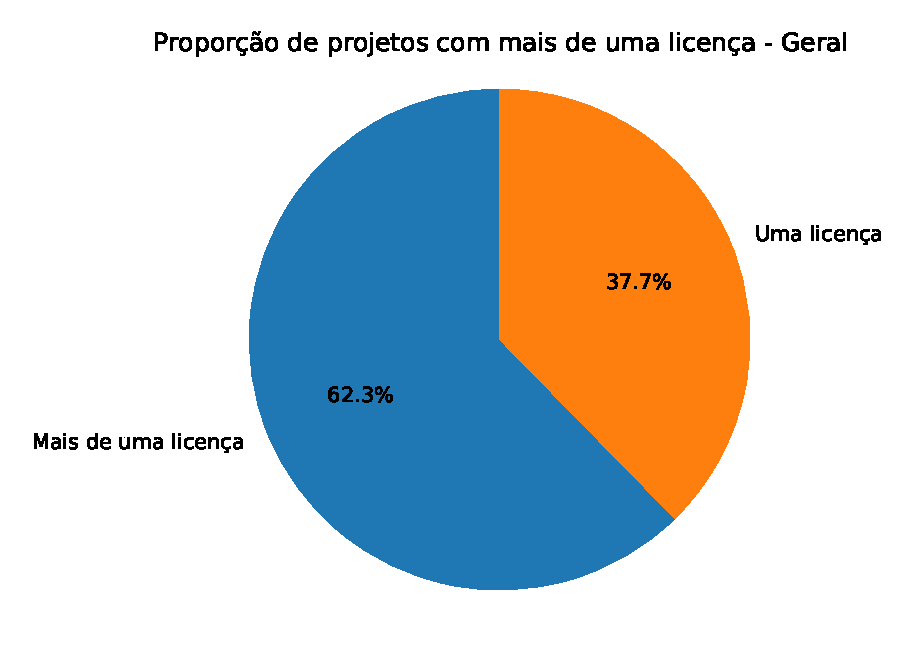
\includegraphics[scale=0.8]{figuras/resultados/pizza_lic_geral.eps}
    \fonte{Autoria própria.}
    \label{local-licencas-raiz}
\end{figure}

A Figura~\ref{local-licencas-raiz} apresenta a proporção de projetos com mais de uma licença. Como pode ser observado, cerca de 38\% dos projetos (582 projetos) apresentam somente uma licença, enquanto que a maioria, mais de 62\% dos projetos (963 projetos), apresenta mais de uma licença. 

%Quando se analisou a quantidade de projetos com mais de uma licença no seu panorama geral, o resultado obtido foi que mais de 60\%  dos analisados apresentaram mais de uma licença contra menos de 40\%.

\begin{figure}[H]
    \centering
    \caption{Proporção de projetos com mais de uma licença - Raiz}
    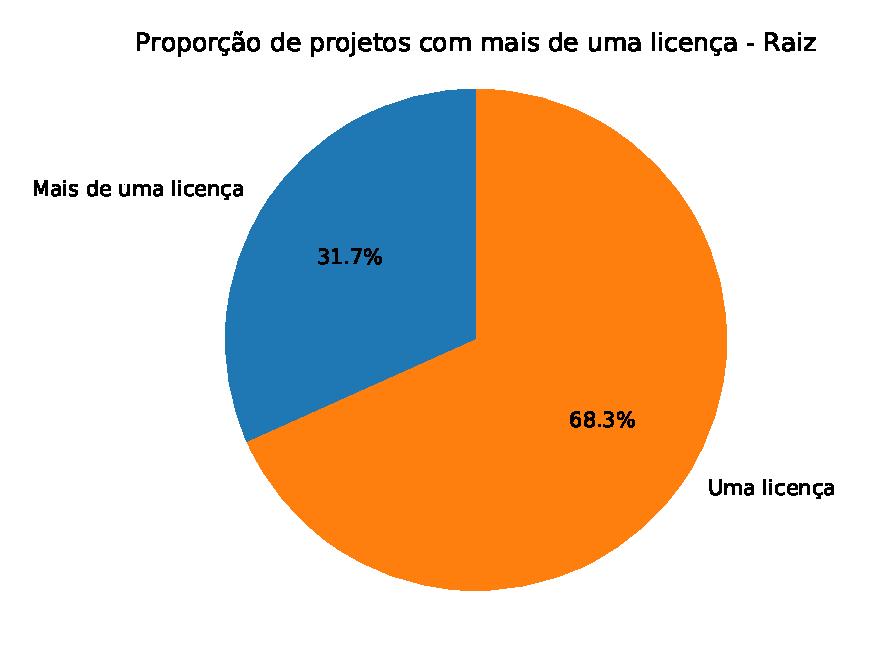
\includegraphics[scale=0.8]{figuras/resultados/pizza_lic_raiz.eps}
    \fonte{Autoria própria.}
    \label{local-licencas-raiz}
\end{figure}

No entanto, é conhecido que desenvolvedores usam diferentes abordagens para declarar licenças de software livre em seus projetos \gnote{citar: http://gustavopinto.org/lost+found/msr2018b.pdf}. Por exemplo \gnote{citar exemplos com detalhes, pe readme, license, outras pastas, etc.}. Dessa forma, foi feito uma nova análise do uso de licenças, mas agora considerando somente as licenças encontradas nas raízes dos projetos. \gnote{mas o label da figura anterior da entender que ela que é na raiz. esse texto é da raiz ou anterior? ajeitar.}
Dessa forma, obtivemos um cenário diferente, onde quase 70\% (1.055 projetos) apresentaram apenas uma licença, ao passo que cerca de 30\% (490 projetos) que apresentam mais de uma licença. Essa análise sugere que desenvolvedores frequentemente não declaram na raiz do projeto todas as licenças utilizadas. Dessa forma, ferramentas que levam em consideração somente licenças declaradas nas raiz potencialmente perdem uma quantidade importante de licenças declaradas em projetos de software livre.

\subsection{Licenças na raiz vs em subdiretórios} \gnote{mover essa subsecao para o local mais adequado}

Para melhor entender o contexto em que licenças são declaradas em subdiretórios dos projetos, foi feita uma análise manual de xxx projetos \gnote{colocar numero}. Após essa análise, foi-se observado três principais principais motivos:

 \begin{itemize}
   \item Muitas das licenças encontradas nos subdiretórios são provenientes de dependências dos projetos. %Com isso licenças de outras projetos.  
   Por exemplo, foi percebido que o projeto tablesaw\footnote{Tablesaw é um projeto do Filament Group que consiste em um conjunto de plugins para criação de tabelas responsivas. Disponível em: \url{https://github.com/filamentgroup/tablesaw/}}, que usa a licença MIT no arquivo LICENSE e no arquivo de package.json, faz uso também da licença Apache\gnote{versao}, no interior de seus diretórios. Isso acontece por causa do uso de bibliotecas externas que foram inseridas no código. Nesse caso em particular, foi adicionado a biblioteca qunit.js, que tem licença MIT e Apache, fazendo com que o projeto tablesaw também adotasse a licença Apache.
   
   \item Licenças provenientes de documentações, como as licenças Creative Commons. Foi percebido que o projeto AngularJs\footnote{AngularJS é um framework JavaScript código aberto, mantido pelo Google, que auxilia na execução de single-page applications. Disponível em: \url{https://github.com/angular/angular}}, usa a licença MIT no arquivo LICENSE e no arquivo de package.json, faz uso também da licença Creative Commons, no interior de seus diretórios. Isso acontece por causa do uso licenças em arquivos de documentação. 
   
   \item Licenças provenientes de exemplos onde o criador especificou uma licença para uso de tal exemplo. Foi percebido que o projeto Gatsby\footnote{Gatsby é um framework gratuito e de código aberto baseado no React que ajuda os desenvolvedores a criar sites e aplicativos rápidos. Disponível em: \url{https://github.com/gatsbyjs/gatsby}}, usa a licença MIT no arquivo LICENSE e no arquivo de package.json, foram encontradas outras licenças MIT no interior de seus diretórios\gnote{nao entendi? ele nao esta usando a mesma licença, mesmo que declarada mais de uma vez? qual o problema?}. Isso acontece por causa do uso licenças em arquivos de exemplo. 
 \end{itemize}

% DISTRIBUIÇÃO DE FREQUENCIA DE LICENÇAS ------------------------------------

\subsection{Quantidade de projetos com mais de uma licença}

Em seguida, foi estudado a proporção de licenças por projeto JavaScript. 
Os resultados da distribuição de frequência estão apresentados na Figura~\ref{local-licencas-raiz}. Nesta figura os outliers foram filtrados para que não ocorra prejuízos na interpretação dos dados. No entanto, os outliers não foram removidos dos dados brutos.

\begin{figure}[H]
    \centering
    \caption{Distribuição de frequência da licenças encontradas em todos os projetos. Outliers foram removidos para que não ocorra prejuízos na interpretação dos dados.}
    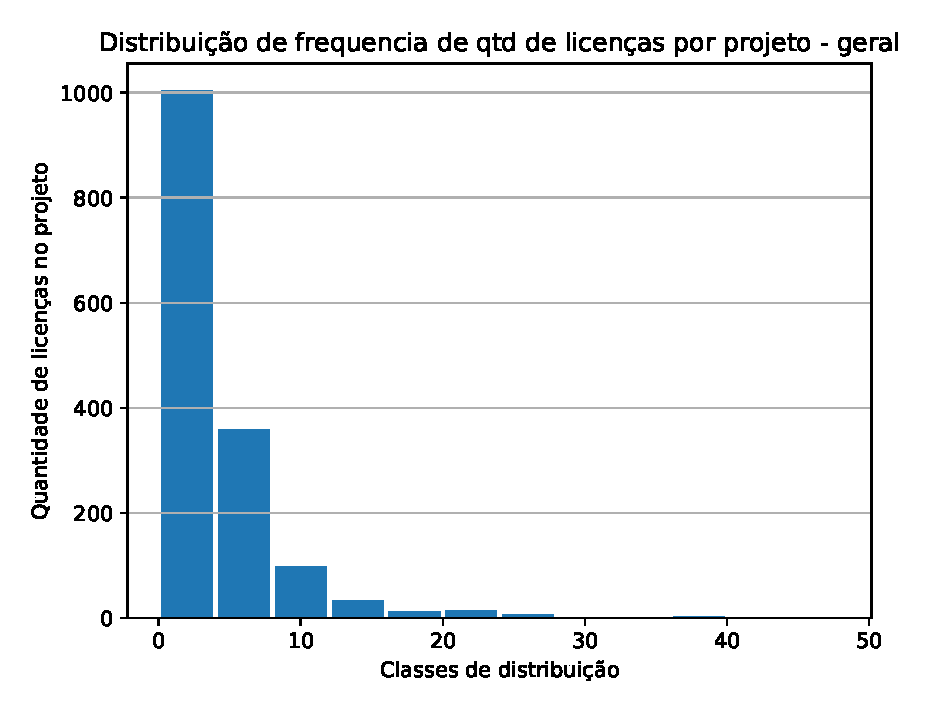
\includegraphics[scale=0.8]{figuras/resultados/hit_qtd_projeto.eps}
    \fonte{Autoria própria.}
    \label{local-licencas-raiz}
\end{figure}


Diante dos resultados observou-se que nas licenças encontradas, no contexto geral de cada projeto analisado, concentra-se entre no intervalo entre 1 e 10 licenças por projeto.\gnote{quantos projetos até 10 licenças?}
No entanto, nesta analise foram encontrados 7 projetos com mais de 50 licenças, entre um intervalo de 86 a 256. Dentre os projetos com mais de 50 licenças, detacam-se xxx (com xxx licenças), xxx (com xxx licenças) e xxx (com xxx licenças).\gnote{complemetnar}

Ademais, estudou-se novamente a distribuição de licenças, considerando somente a declaração de licenças feitas na raiz do projeto. 
Já nessa analise foram encontrados apenas 19 projetos com mais de 7 licenças, reforçando o achado anterior que apresentou que muitas licenças de software livre não são declaradas na raiz do projeto. 
%Compreendendo um intervalo entre 8 e 43 licenças por projeto, com isso esses valores foram removidos como outlier para facilitar a visualização dos dados. 
Nesse contexto, observou-se que existe uma grande concentração de projetos entre o intervalo entre 1 e 2 licenças.\gnote{quantos projetos até 2 licenças?}

\begin{figure}[H]
    \centering
    \caption{Distribuição de frequência da licenças encontradas apenas na raiz dos projetos}
    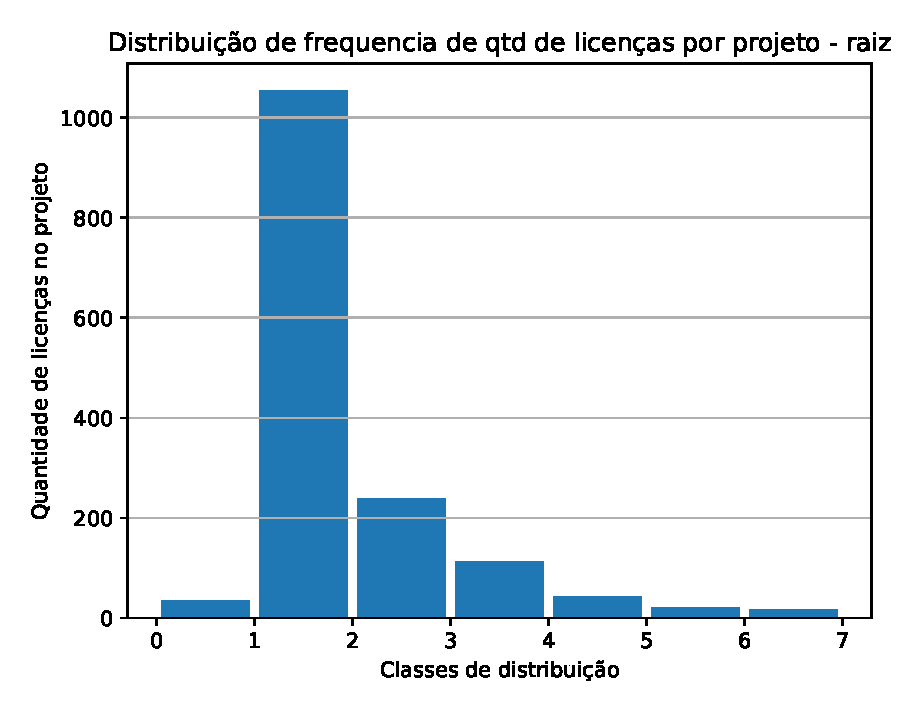
\includegraphics[scale=0.8]{figuras/resultados/hit_qtd_raiz.eps}
	\fonte{Autoria própria.}
    \label{local-licencas-raiz}
\end{figure}


\subsection{Uso de licença não-software} 

%\section{Qual o quantitativo de licenças (de software e não-software) encontradas nos projetos?}

Como foi observado anteriormente, uma parte das licenças encontradas em sub-diretórios não era licença de software (como a Creative Commons). Para melhor entender a existência e uso dessas licenças, foi feito uma uma analise para categorizar as licenças como (1) licenças de software e (2) não-software (licenças de documentação, patente, etc). Para definir as licenças de software, foi utilizado os sites xxx e yyy que fornecem essa descrição, bla bla bla\gnote{complementar}. A Figura~\ref{local-licencas-raiz} apresenta o resultado encotnrado.



\begin{figure}[H]
    \centering
    \caption{quantitativo de licenças (de software e não software) - Geral}
    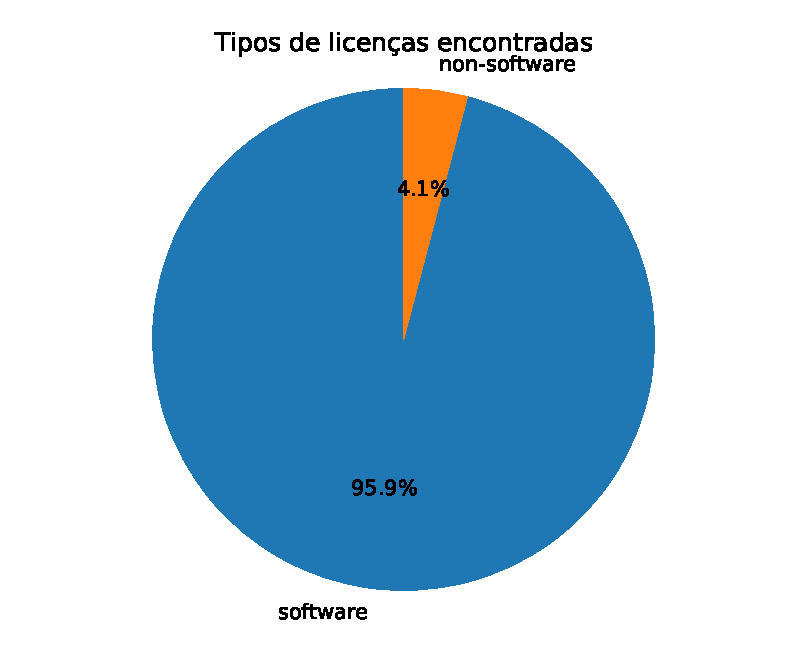
\includegraphics[scale=0.8]{figuras/resultados/tipos_licenca.eps}
    \fonte{Autoria própria.}
    \label{local-licencas-raiz}
\end{figure}

Como se pode observar,  mais de 95\% (248.596 licenças) dos analisados são licenças de software contra apenas de 5\% (10.618 licenças) sendo licenças categorizadas como sendo não-software. Dentre as principais licenças de não-software encontradas, destacam-se as licenas xxx (xxx ocorrencias), xxx (xxx ocorrencias) e xxx (xxx ocorrencias). \gnote{descrever}


% LOCALIZAÇÃO DAS LICENÇAS ---------------------------------------------------
\section{Onde desenvolvedores declaram as licenças?}

Com o intuito de esclarecer os principais arquivos onde foram encontrada as licenças de software livre, foi agrupados os resultados em três arquivos: o license, o readme, e o package.json. O license, como seu nome sugere, é o arquivo principal, no que se refere a declaração de licenças de software livre. Seu uso é extremamente difundido \gnore{citação} e sítios como o GitHub automaticamente inferem estes arquivos para identificar as licenças descritas. O arquivo readme, por outro lado, apresenta uma descrição geral do projeto, geralmente para novos desenvolvedores que querem se ambientar e/ou contribuir com o projeto. Este arquivo também é frequentemente utilizado para declarar as licenças de um projeto, embora não seja necessáriamente obrigatório \gnote{leia a introducao esse arquivo: e melhore o texto como necesario https://ctreude.files.wordpress.com/2018/09/emse18.pdf}. Por fim, o arquivo package.json é a porta de entrada do sistema de gerenciador de pacotes NPM. Além da licença, esse arquivo declara informações como xxx \gnote{complementar}. Se uma licença for declarada, após o deploy do pacote no NPM, os usuários que navegam pelo sítio do NPM poderão identificar o uso dessa licença diretamente no sitio, sem precisarem navegar pelo código fonte ou acessar outros sites (como o GitHub). Em todos os casos, é responsabilidade do mantenedor de projetos adicionar as informações de licença nesses arquivos.
A Figura~\ref{local-licencas-raiz} apresenta a distribuição das licenças entre os arquivos mencionados. Ainda, é apresentado uma barra com ''outros'', o que significa a declaração da licença em outros arquivos.

\begin{figure}[H]
    \centering
    \caption{localização das licenças encontradas na raiz dos projetos}
    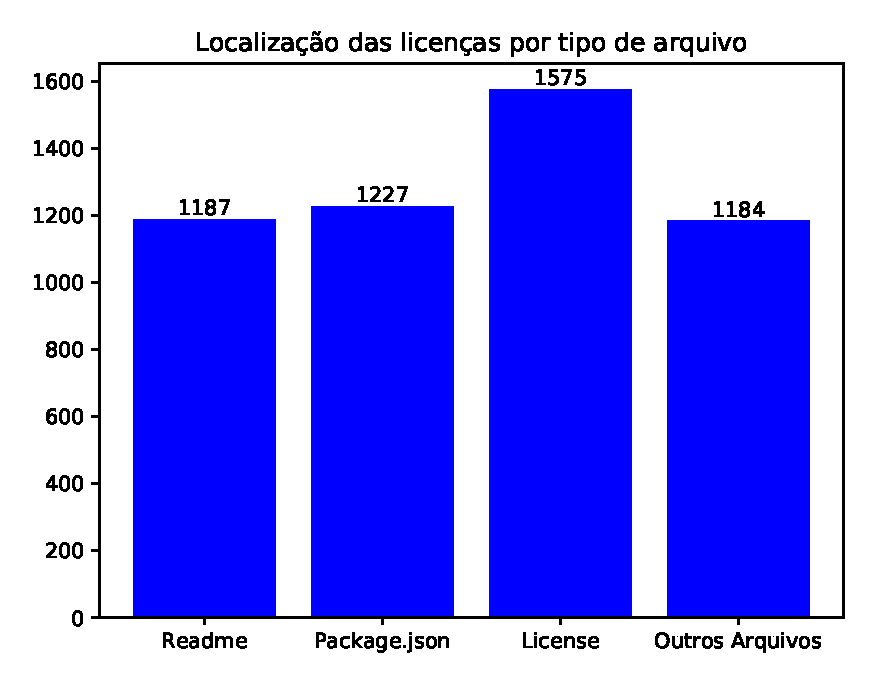
\includegraphics[scale=0.8]{figuras/resultados/barras_local_licencas.eps}
	\fonte{Autoria própria.}
    \label{local-licencas-raiz}
\end{figure}

Como observa-se, a maioria das licenças foram encontradas em arquivos do tipo ``license". Pode se observar também, que essa quantidade é superior a quantidade de projetos analisados, pois existem projetos que apresentam mais de uma licença e cada licença é listada em um arquivo individual. Como um exemplo, detaca-se o projeto Annotator\footnote{Annotator é uma biblioteca JavaScript para criar aplicativos de anotação em navegadores. Ele fornece um conjunto de ferramentas interoperáveis para anotar conteúdo em páginas da web. Link do projeto: \url{https://github.com/openannotation/annotator}}, que apresenta a licença MIT em um arquivo nomeado "LICENSE-MIT" e a licença GLP em um outro arquivo "LICENSE-GPL".

Com relação aos outros arquivos, foi observado que arquivos como xxx e yyy são frequentemente utilizados para declarar licenças \gnote{aqui seria bom achar outros arquivos famosos, e menciona-los no texto}.


% LICENÇAS CONHECIDAS ---------------------------------------------------
\section{Com que frequência são feitas violações no uso de licenças?}

Há várias formas de desenvolvedores violarem uso de licenças, como xxx ou yyy. Particularmente importante para esse trabalho, estamos interessados no uso de licenças que não foram formalmente aprovadas por uma entidade (Seção~\ref{sec:spdx}), além do uso irrestrito de licenças permissivas e restritivas (Seção~\ref{sec:comp}).

\gnote{aqui usa-se somente os projetos com 2 mais licenças? em outros lugares tbm? precisa deixar isso claro no texto.}

\subsection{Uso de licenças não reconhecidas pela SDPX}\label{sec:spdx}

Nessa parte do trabalho, foi analisado o uso de licenças conhecidas e não conhecidas pela SPDX. O Software Package Data Exchange® (SPDX®) é um padrão aberto para a comunicação de informações da lista de materiais de software (incluindo componentes, licenças, direitos autorais e referências de segurança). A especificação SPDX é desenvolvida pelo grupo de trabalho SPDX, hospedado pela The Linux Foundation. Para cada licença encontrada, foi observado se essa licença está descrita no site da SPDX de licenças conhecidas\footnote{https://spdx.org/licenses/}.

\begin{figure}[H]
    \centering
    \caption{Proporção do uso de licenças SPDX}
    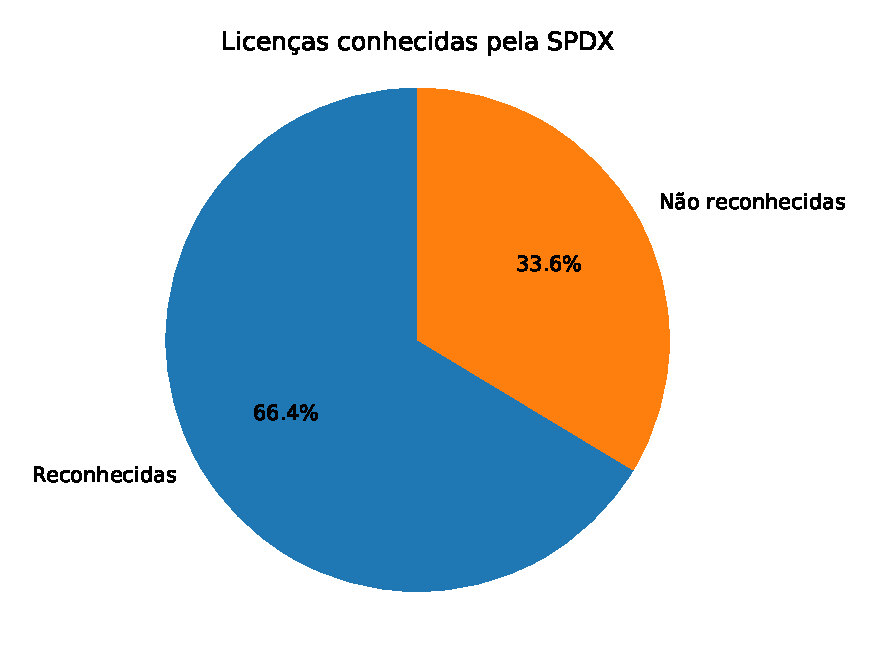
\includegraphics[scale=0.8]{figuras/resultados/pizza_licencas_conhecidas.eps}
	\fonte{Autoria própria.}
    \label{local-licencas-raiz}
\end{figure}

Como é possível observar, mais de 65\% (288 licenças) das licenças encontradas nos projeto são reconhecidas pela SPDX contra cerca de 35\% (146 licenças) não foram reconhecidas pela SPDX. \gnote{pq esses numeros nao abtem no numero total de licencas? descrever no texto} 

\gnote{descrever aqui as licenças não reconhecidas. quais sao? ao menos as tres mais utilizadas}

% COMPATIBILIDADE DE LICENÇAS ---------------------------------------------------
\subsection{Qual a quantitativo de licenças permissivas e restritivas?}\label{sec:comp}

Por fim, foi feita uma análise com o intuito de esclarecer o quantitativo de licenças permissivas e restritivas. Por licenças restritivas, entende-se \gnote{complementar}. Por licenças restritivas, entende-se \gnote{complementar}. Figure~\ref{local-licencas-raiz} apresenta os resultados.

\gnote{aqui tem que descrever melhor.. nao é o caso em que *no mesmo projeto* sao utilizados dois tipos de licenças diferentes? descreva como isso foi feito...}

\begin{figure}[H]
    \centering
    \caption{Compatibilidade de licenças encontradas no projeto}
    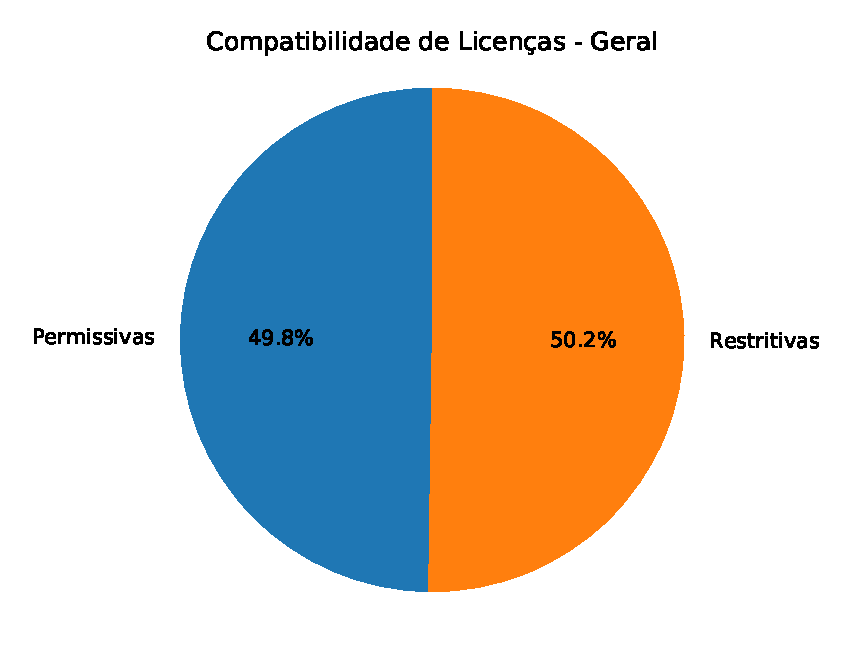
\includegraphics[scale=0.8]{figuras/resultados/pizza_compatibilidade_geral.eps}
	\fonte{Autoria própria.}
    \label{local-licencas-raiz}
\end{figure}

Rastreando todas as licenças encontradas no projeto de forma geral (licenças na raiz e em diretórios secundários), observou um empate em quantitativo de licenças que são compatíveis e não compatíveis nos projetos. Sendo que 50,5\% (780 licenças) permissivas e 49,5\% (765 licenças) são restritivas.

\begin{figure}[H]
    \centering
    \caption{Compatibilidade de licenças encontradas na raiz do projeto}
    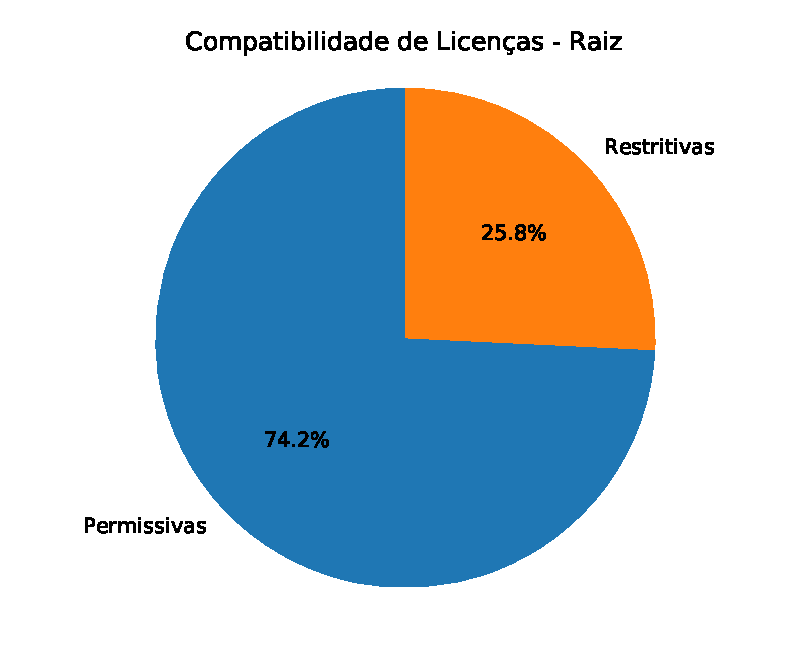
\includegraphics[scale=0.8]{figuras/resultados/pizza_compatibilidade_raiz.eps}
	\fonte{Autoria própria.}
    \label{local-licencas-raiz}
\end{figure}

Quando a busca foi restrita apenas as licenças encontradas na raiz dos projetos o panorama mudou, pois apenas 25\% das licenças encontradas eram incompatíveis. Sendo que 76,3\% (1.179 licenças) são compatíveis e 23,7\% (366 licenças) não são compativeis.

%comentario inicial=====================
\begin{comment}

% CATEGORIA DAS LICENÇAS ---------------------------------------------------
\section{Como as licenças encontradas podem ser categorizadas?}
Foi analisado os resultados da ferramenta com o intuito de esclarecer o tipo das licenças encontradas. Com essa analise podemos observar que a maioria das licenças são do tipo permissiva

\begin{table}[h]
	\centering
	\caption{Categoria das licenças encontradas.}
	\label{tab:categiorias}	
	    \begin{tabular}{l c c}
        \hline Categorias & Quantitativo Absoluto & Quantitativo Percentual (\%)\\
        \hline        
Permissive                & 193.899                & 74,80                          \\
Unstated License          & 19.202                 & 7,41                          \\
Copyleft Limited          & 14.290                 & 5,51                         \\
Patent License            & 10.634                 & 4,10                       \\
Copyleft                  & 10.257                 & 3,96                     \\
Source-available          & 7.194                  & 2,78                  \\
Public Domain             & 2.826                  & 1,09                  \\
Proprietary Free          & 809                    & 0,31                       \\
Free Restricted           & 52                     & 0,02                        \\
        \hline
Total                     & 259.214                & 100,00                      \\
        \hline
    \end{tabular}
	\fonte{Autoria própria.}
\end{table}


As licenças encontradas foram categorizadas conforme metodologia da ferramentas, essas categorias tem os seguintes significados:

\subsection {Permissive}
Software de código aberto disponibilizado sob licenças "não copyleft".
Isso geralmente exige a atribuição do código aberto incluído e pode incluir outras obrigações.

\subsection {Unstated License}
Software de terceiros com aviso de direitos autorais, mas sem licença declarada.
Exemplos comuns incluem trechos de código de publicações e sites (como os da O'Reilly Media).
A ausência de uma licença representa um risco de que o proprietário dos direitos autorais possa reivindicar obrigações de licença em algum momento futuro.
As equipes de produtos podem precisar entrar em contato com o proprietário dos direitos autorais para determinar as obrigações de licença, se houver.
Nessa categoria de licencas foram encontradas as seguintes licenças:

\subsection {Copyleft Limited}
Uma licença que exige que você redistribua o código-fonte, incluindo suas alterações, e também forneça atribuição aos autores do software.
Sua obrigação de redistribuir o código-fonte, incluindo o código proprietário vinculado ao código sob esta licença, é limitada de acordo com as regras específicas da licença.
Nessa categoria de licencas foram encontradas as seguintes licenças:

\subsection {Patent License}
Uma licença que se aplica a patentes em vez de software específico.
Pode ser usado em conjunto com outras licenças de software que se aplicam a um componente de software

\subsection {Copyleft}
Software de código aberto com uma licença "copyleft" que oferece permissão irrevogável ao público para copiar e redistribuir o trabalho da mesma forma ou modificado, mas com as condições em que todas essas redistribuições disponibilizam o trabalho em um formato que facilita modificações e uso adicionais os mesmos termos da licença.
Uma licença copyleft pode exigir que o código que interage com o código licenciado copyleft seja licenciado da mesma maneira.

\subsection {Source-available}
O software disponível na fonte é um software liberado por meio de um modelo de distribuição de código-fonte que inclui disposições em que a fonte pode ser visualizada e, em alguns casos, modificada, mas sem necessariamente atender aos critérios a serem chamados de fonte aberta.

\subsection {Public Domain}
Software de código aberto disponibilizado sem obrigações explícitas, mas com um aviso de licença que deve ser mantido com o código por política da organização.
A correspondência pode ser com software, exemplos de código em um site, especificações de domínio público publicadas ou outro tipo de publicação

\subsection {Proprietary Free}
Software gratuito proprietário que pode não exigir uma licença comercial, mas pode ter termos e condições específicos que as equipes de produto são obrigadas a seguir.
Alguns desses termos e condições são fornecidos com ou no código ou em licenças baixadas clicáveis.
Exemplos são o Contrato de Licença de Código Binário da Sun ou um BSP oferecido gratuitamente.

\subsection {Free Restricted}
Uma licença de estilo permissivo, que contém restrições sobre o uso do software (por exemplo, quando o software não se destina ao uso em usinas nucleares) ou o
redistribuição do software (por exemplo, onde a redistribuição comercial do software não é permitida sem permissão expressa).
A Free Software Foundation (FSF) diz que uma licença com esse tipo de restrição não é realmente de código aberto, embora o ponto de vista da OSI não seja tão rigoroso.

\end{comment}
%comentario final =====================
	% REVISÃO DE LITERATURA--------------------------------------------------------

\chapter{TRABALHOS RELACIONADOS}
\label{chap:fundamentacaoTeorica}
Sera feita uma analise de trabalhos relacionados de outros autores sobre o tema de trabalho, dentro desse cenário vasto do licenciamento de software, sera abordado trabalho que tange a temática abordada nesse trabalho de conclusão.

No artigo \cite{Vendome:2018:DDW:3180155.3180221} é explanado como os erros de licenciamento de software são importantes, pois com a variedade de licencias de software (restritivas e permissivas) existentes podem ser criadas confusões na hora do licenciamento do software, que não necessariamente limitam a compatibilidade das licenças. Esse estudo é resultado de uma analise manual de 1.200 discussões relacionadas a erros de licenciamento realizadas em issue trackers e em cinco mailing lists de discussões de projeto da comunidade open source. 

Neste trabalho notou-se que os erros de licenciamento se dão por motivos diversos, pois compreendeu-se que as leis de direitos autorais são complexas para a maioria dos desenvolvedores. Foi observado também que em alguns projetos de código aberto, existe a discussão em termos de se uma ação tem o potencial de violar direitos autorais, onde geralmente essas discussões estão entre os desenvolvedores, que não necessariamente tem o entendimento adequado da lei de direitos autorais e geralmente não tem aconselhamento jurídico profissional. 

No artigo \cite{Meloca:2018:UUI:3196398.3196427} é abordada uma questão importante no cenário de licenciamento de software que é negligenciada: o uso de licenças de de código aberto, mas que não foram formalmente aprovadas pela Open Source Iniative (OSI), pois quando um desenvolvedor lança um software sob uma licenças não aprovada, mesmo que o interesse seja torna-lo de código aberto, o  autor pode não esta concedendo os direitos exigidos para aqueles que usam o software. 

Para descobrir as razões por trás desse uso forma minerados dados de 675k projetos de código aberto e suas versões, e também 76 desenvolvedores que publicaram alguns desses projetos. O estudo foi realizado e varias características foram observadas. Como que não é incomum para desenvolvedores mudarem a licenças não aprovadas para licenças aprovadas pela OSI, que quando os desenvolvedores foram questionados sobre a mudança os mesmo mencionaram que que essa transição foi devido a uma melhor compreensão das desvantagens do uso de uma licença aprovadas, mostrando mais uma vez que essa parte de licenciamento de software necessita de um maior esclarecimento de como as licencias funcionam para o desenvolvedores desses projetos.

Em cerca de 24\% dos projetos analisados, observou-se que usavam pelo menos uma licença não aprovada pela OSI, sendo que a maioria dessas licenças não aprovadas eram projetos sem licença alguma. Quando o estudo entrou em contato com os mantenedores dos projetos, 46\% dos entrevistados não levam em consideração a licença quando escolhem uma dependência de pacote e alguns entrevistados acreditam que as licenças não aprovadas são mais abertas e mais simples de usar.

No artigo \cite{Vendome:2017:LUC:3106879.3106907} é feito um extenso estudo empírico, em larga escala no gitHub, sobre alterações de licenças. Foi feita uma investigação de caráter qualitativa e quantitativa de quanto e por que os desenvolvedores adotam ou alteram as licenças dos softwares. Na analise feita nas mensagens de commits e nas discussões de issues destacou-se que as informações oferecidas com relação à escolhas/alterações do licenciamento geralmente são bastantes limitadas, com isso um desenvolvedor interessado em reutilizar o código seria forçado a verificar o código fonte para entender o licenciamento exato ou solicitar esclarecimento. Além disso, os motivos por trás da alteração geralmente não são bem documentados, mas notou-se uma tendencia em alterações de licenciamento predominantemente em direção ou entre licenças permissivas, que facilitam algum tipo de trabalho derivado e redistribuição, por exemplo, em produtos comerciais.

Foi observado também que os desenvolvedores interpretam as implicações do licenciamento de maneira diferente, o que gera mal-entendidos nos termos de reutilização, culminando em uma reutilização de código problemática para os desenvolvedores devido ao licenciamento

A falta de padronização na maneira como a documentação do licenciamento é expresso nos projetos também foi um problema observado, visto que alguns projetos apresentavam a licenças no diretório pai, outras no cabeçalho do código fonte. Assim com foi observado que o uso comercial dos projetos é uma preocupação da comunidade, mostrando assim a importância de licenças como MIT e Apache para esses fins, que aparecem com bastante frequência nos projetos open source atualmente.

No artigo \cite{BSDeMIT} foi apresentado um estudo empírico de como as famílias de licenças BSD e MIT variam de sua definição original. A família de licenças BSD se aproxima dos modelos SPDX existentes, com pouca variabilidade adicional. A família de licenças MIT foi encontrado para ser muito mais fragmentado e altamente personalizado, incluindo a criação de várias variantes especializadas baseadas na licença original do X11, personalização do texto "autores ou detentores de direitos autorais", alterações ortográficas e adição e remoção de condições, subsídios e sentenças completas. Pequenas alterações no modelo SPDX para o Licença MIT e à lista SPDX de palavras equivalentes acomodariam algumas a variação essencial encontrada na licença a um baixo custo.

Observou-se que os licenciadores alteram o texto das licenças padrão de código aberto para vários propósitos, incluindo a personalização da licença com o nome de sua organização específica, adicionando ou removendo condições e alteração de ortografia ou pontuação. Padrões de licenciamento de código aberto, como O SPDX pode ser afetado pela variabilidade nas licenças, pois a variabilidade pode alterar os requisitos legais. significado das licenças, criando problemas legais na correspondência de uma licença alterada. Em contraste, a exigência de uma "combinação perfeita" excessivamente rigorosa de licenças de código aberto para o padrão pode resultam na exclusão de muitos textos de licença com variabilidade insignificante. 
	% AMEAÇAS A VALIDADE--------------------------------------------------------

\chapter{AMEAÇAS A VALIDADE DO TRABALHO}
\label{chap:AmeacasAValidade}

%\section{Validação de Construção}
As ameaças para construir a validade do trabalho dizem respeito à relação entre teoria e observação, e relacionam-se a uma possível imprecisão da medição ao extrair dados usados neste estudo. Os resultados ficam intimamente ligados a acurácia e limitações da ferramenta utilizada para gerar os dados para analise.

%\section{Validação Interna}
%\section{Validação Externa}
Ameaças à validade externa representam a capacidade de generalizar as observações em nosso estudo. Nosso estudo quantitativo é baseado na análise de mais de 1.500 repositórios hospedados no Github da linguagem Javascript.  No entanto, a generalização de nossos resultados qualitativos é limitada a linguagem Javascript escolhida no dataset que podem não espelhar o verdadeiro cenário da população completa de repositórios hospedados no Github.
%\section{Confiabilidade}


\begin{comment}
 Na mineração dos repositórios Git, contamos com a API GitHub e a linha de comando git
utilitário. Essas são as duas ferramentas em desenvolvimento ativo e têm um apoio comunitário
eles. Além disso, a API do GitHub é a interface principal para extrair informações do projeto.
Não podemos excluir imprecisões devido à implementação dessa API. Em termos de licença
Na classificação, contamos com Ninka, uma abordagem de ponta que demonstrou ter
95% de precisão (German et al., 2010b); no entanto, nem sempre é capaz de identificar o
licença (15% do tempo nesse estudo). No que diz respeito à codificação aberta realizada em
No contexto do RQ4, identificamos, por meio de uma amostra estratificada, uma amostra de confirmação
mensagens e discussões de rastreadores de problemas grandes o suficiente para garantir um erro de ± 10% com um
nível de confiança de 95%. Essa amostra foi identificada a partir da confirmação do candidato
mensagens e discussões identificadas por meio da correspondência de padrões, usando as palavras-chave
Tabela 1. Embora tenhamos como objetivo criar um conjunto abrangente de palavras-chave relacionadas ao licenciamento, é
é possível que tenhamos perdido discussões relacionadas ao licenciamento que não correspondam a nenhuma dessas palavras-chave.

Ameaças à validade interna podem estar relacionadas a fatores de confusão internos ao nosso estudo,
isso poderia ter afetado os resultados. Para as alterações no licenciamento atômico, reduzimos a ameaça
de ter o tamanho do projeto como um fator de confusão, representando as presenças de uma alteração específica em cada confirmação. Uma alteração de licença geralmente é tratada em uma determinada instância e não
frequência. Ao usar a análise no nível de confirmação, impedimos que o número de arquivos seja inflado
os resultados para que eles não sugiram inadequadamente um grande número de alterações ocorridas
em um projeto. Para analisar as mudanças entre os projetos, adotamos uma abordagem binária de analisar a presença de um padrão. Portanto, um projeto em particular não dominaria nossos resultados
devido ao tamanho. Para limitar a subjetividade da codificação aberta, as classificações sempre foram realizadas por dois dos autores e, em seguida, todos os casos de classificação discográfica foram discutidos.
conforme explicado na Seção 3.3.

 No entanto, a generalização de nossos resultados qualitativos é limitada aos sete idiomas considerados e é
suportado pelo número relativamente baixo de sistemas considerados (ou seja, 1.160) devido ao manual
esforço necessário para identificar a lógica por trás das decisões de licenciamento (bem como
o número limitado de repositórios em potencial com mensagens de confirmação ou problemas relacionados à licença
discussões).
O crescimento exponencial e a popularidade do GitHub como forja pública indicam que ele representa
uma grande parte da comunidade de código aberto. Enquanto o crescimento exponencial ou relativo
Como a juventude dos projetos pode impactar os dados, essas duas características representam a
crescimento do desenvolvimento de código aberto e não deve ser descartado. Além disso, o GitHub
contém um grande número de repositórios, mas pode não ser necessariamente um
conjunto de todos os projetos de código aberto ou mesmo todos os projetos Java. Contudo, o grande número de
projetos em nosso conjunto de dados (e valores de métricas de diversidade relativamente altos, como mostrado na Seção 3.4)
nos dá confiança suficiente sobre as descobertas obtidas. Avaliação adicional dos projetos

\end{comment}
	%% ORIENTAÇÕES GERAIS------------------------------------------------------------


% SOBRE AS ILUSTRAÇÕES----------------------------------------------------------
\chapter{SOBRE AS ILUSTRAÇÕES}
\label{chap:apSobreIlust}

A seguir exemplifica-se como inserir ilustrações no corpo do trabalho. As ilustrações serão indexadas automaticamente em suas respectivas listas. A numeração sequencial de figuras, tabelas e equações também ocorre de modo automático.

Referências cruzadas são obtidas através dos comandos \verb|\label{}| e \verb|\ref{}|. Sendo assim, não é necessário por exemplo, saber que o número de certo capítulo é \ref{chap:fundamentacaoTeorica} para colocar o seu número no texto. Outra forma que pode ser utilizada é esta: \autoref{chap:fundamentacaoTeorica}, facilitando a inserção, remoção e manejo de elementos numerados no texto sem a necessidade de renumerar todos esses elementos.

% FIGURAS-----------------------------------------------------------------------
\chapter{FIGURAS}
\label{chap:figuras}

Exemplo de como inserir uma figura. A \autoref{fig:figura-exemplo1} aparece automaticamente na lista de figuras. Para saber mais sobre o uso de imagens no \LaTeX{} consulte literatura especializada \cite{Goossens2007}.

Os arquivos das figuras devem ser armazenados no diretório de "/dados".

\begin{figure}[!htb]
    \centering
    \caption{Exemplo de Figura}
    \includegraphics[width=0.5\textwidth]{./dados/figuras/figura1}
    \fonte{\citeonline{IRL2014}}
    \label{fig:figura-exemplo1}
\end{figure}

% QUADROS E TABELAS---------------------------------------------------------------
\chapter{QUADROS E TABELAS}
\label{chap:tabelas}

Exemplo de como inserir o \autoref{qua:quadro-exemplo1} e a \autoref{tab:tabela-exemplo1}. Ambos aparecem automaticamente nas suas respectivas listas. Para saber mais informações sobre a construção de tabelas no \LaTeX{} consulte literatura especializada \cite{Mittelbach2004}.

Ambos os elementos (Quadros e Tabelas) devem ser criados em arquivos separados para facilitar manutenção e armazenados no diretório de "/dados".

\input{./dados/quadros/quadro1}

A diferença entre quadro e tabela está no fato que um quadro é formado por linhas horizontais e verticais. Deve ser utilizado quando o conteúdo é majoritariamente não-numérico. O número do quadro e o título vem acima do quadro, e a fonte, deve vir abaixo. E Uma tabela é formada apenas por linhas verticais. Deve ser utilizada quando o conteúdo é majoritariamente numérico. O número da tabela e o título vem acima da tabela, e a fonte, deve vir abaixo, tal como no quadro.

\input{./dados/tabelas/tabela1}

% EQUAÇÕES-----------------------------------------------------------------------
\chapter{EQUAÇÕES}
\label{chap:equacoes}

Exemplo de como inserir a \autoref{eq:equacao-exemplo1} e a Eq. \ref{eq:equacao-exemplo2} no corpo do texto \footnote{Deve-se atentar ao fato de a formatação das equações ficar muito boa esteticamente.}. Observe que foram utilizadas duas formas distintas para referenciar as equações.

\begin{equation}
    X(s) = \int\limits_{t = -\infty}^{\infty} x(t) \, \text{e}^{-st} \, dt
    \label{eq:equacao-exemplo1}
\end{equation}

\begin{equation}
    F(u, v) = \sum_{m = 0}^{M - 1} \sum_{n = 0}^{N - 1} f(m, n) \exp \left[ -j 2 \pi \left( \frac{u m}{M} + \frac{v n}{N} \right) \right]
    \label{eq:equacao-exemplo2}
\end{equation}

% ALGORITMOS-----------------------------------------------------------------------
\chapter{ALGORITMOS}
\label{chap:algoritmos}

Exemplo de como inserir um algoritmo. Para inserção de algoritmos utiliza-se o pacote {\ttfamily algorithm2e} que já está devidamente configurado dentro do template.

Os algoritmos devem ser criados em arquivos separados para facilitar manutenção e armazenados no diretório de "/dados".\\
\\

\input{./dados/algoritmos/algoritmo1}

% SOBRE AS LISTAS--------------------------------------------------------------------
\chapter{SOBRE AS LISTAS}
\label{chap:apSobreLista}

Para construir listas de "\textit{bullets}"{} ou listas enumeradas, inclusive listas aninhadas, é utilizado o pacote \verb|paralist|.

Exemplo de duas listas não numeradas aninhadas, utilizando o comando \verb|\itemize|. Observe a indentação, bem como a mudança automática do tipo de "\textit{bullet}"{} nas listas aninhadas.

\begin{itemize}
    \item item não numerado 1
    \item item não numerado 2
    \begin{itemize}
        \item subitem não numerado 1
        \item subitem não numerado 2
        \item subitem não numerado 3
    \end{itemize}
    \item item não numerado 3
\end{itemize}

Exemplo de duas listas numeradas aninhadas, utilizando o comando \verb|\enumerate|. Observe a numeração progressiva e indentação das listas aninhadas.

\begin{enumerate}
    \item item numerado 1
    \item item numerado 2
    \begin{enumerate}
        \item subitem numerado 1
        \item subitem numerado 2
        \item subitem numerado 3
    \end{enumerate}
    \item item numerado 3
\end{enumerate}

% SOBRE AS CITAÇÕES E CHAMADAS DE REFERÊNCAS----------------------------------------------
\chapter{SOBRE AS CITAÇÕES E CHAMADAS DE REFERÊNCAS}
\label{chap:apSobreCita}

Citações são trechos de texto ou informações obtidas de materiais consultadss quando da elaboração do trabalho. São utilizadas no texto com o propósito de esclarecer, completar e embasar as ideias do autor. Todas as publicações consultadas e utilizadas (por meio de citações) devem ser listadas, obrigatoriamente, nas referências bibliográficas, para preservar os direitos autorais. São classificadas em citações indiretas e diretas.

% CITAÇÕES INDIRETAS-----------------------------------------------------------------------
\chapter{CITAÇÕES INDIRETAS}
\label{chap:citacoesLivres}

É a transcrição, com suas próprias palavras, das idéias de um autor, mantendo-se o sentido original. A citação indireta é a maneira que o pesquisador tem de ler, compreender e gerar conhecimento a partir do conhecimento de outros autores. Quanto à chamada da referência, ela pode ser feita de duas maneiras distintas, conforme o nome do(s) autor(es) façam parte do seu texto ou não. Exemplo de chamada fazendo parte do texto:\\
\\Enquanto \citeonline{Maturana2003} defendem uma epistemologia baseada na biologia. Para os autores, é necessário rever \ldots.\\

A chamada de referência foi feita com o comando \verb|\citeonline{chave}|, que produzirá a formatação correta.

A segunda forma de fazer uma chamada de referência deve ser utilizada quando se quer evitar uma interrupção na sequência do texto, o que poderia, eventualmente, prejudicar a leitura. Assim, a citação é feita e imediatamente após a obra referenciada deve ser colocada entre parênteses. Porém, neste caso específico, o nome do autor deve vir em caixa alta, seguido do ano da publicação. Exemplo de chamada não fazendo parte do texto:\\
\\Há defensores da epistemologia baseada na biologia que argumentam em favor da necessidade de \ldots \cite{Maturana2003}.\\

Nesse caso a chamada de referência deve ser feita com o comando \verb|\cite{chave}|, que produzirá a formatação correta.

% CITAÇÕES DIRETAS-----------------------------------------------------------------------
\chapter{CITAÇÕES DIRETAS}
\label{chap:citacoesLiterais}

É a transcrição ou cópia de um parágrafo, de uma frase, de parte dela ou de uma expressão, usando exatamente as mesmas palavras adotadas pelo autor do trabalho consultado.

Quanto à chamada da referência, ela pode ser feita de qualquer das duas maneiras já mencionadas nas citações indiretas, conforme o nome do(s) autor(es) façam parte do texto ou não. Há duas maneiras distintas de se fazer uma citação direta, conforme o trecho citado seja longo ou curto.

Quando o trecho citado é longo (4 ou mais linhas) deve-se usar um parágrafo específico para a citação, na forma de um texto recuado (4 cm da margem esquerda), com tamanho de letra menor e espaçamento entrelinhas simples. Exemplo de citação longa:
\\\begin{citacao}
    Desse modo, opera-se uma ruptura decisiva entre a reflexividade filosófica, isto é a possibilidade do sujeito de pensar e de refletir, e a objetividade científica. Encontramo-nos num ponto em que o conhecimento científico está sem consciência. Sem consciência moral, sem consciência reflexiva e também subjetiva. Cada vez mais o desenvolvimento extraordinário do conhecimento científico vai tornar menos praticável a própria possibilidade de reflexão do sujeito sobre a sua pesquisa \cite[p.~28]{Silva2000}.
\end{citacao}

Para fazer a citação longa deve-se utilizar os seguintes comandos:
\begin{verbatim}
\begin{citacao}
<texto da citacao>
\end{citacao}
\end{verbatim}

No exemplo acima, para a chamada da referência o comando \verb|\cite[p.~28]{Silva2000}| foi utilizado, visto que os nomes dos autores não são parte do trecho citado. É necessário também indicar o número da página da obra citada que contém o trecho citado.

Quando o trecho citado é curto (3 ou menos linhas) ele deve inserido diretamente no texto entre aspas. Exemplos de citação curta:\\
\\A epistemologia baseada na biologia parte do princípio de que "assumo que não posso fazer referência a entidades independentes de mim para construir meu explicar" \cite[p.~35]{Maturana2003}.\\
\\A epistemologia baseada na biologia de \citeonline[p.~35]{Maturana2003} parte do princípio de que "assumo que não posso fazer referência a entidades independentes de mim para construir meu explicar".

% DETALHES SOBRE AS CHAMADAS DE REFERÊNCIAS---------------------------------------------------------
\chapter{DETALHES SOBRE AS CHAMADAS DE REFERÊNCIAS}
\label{chap:referUtilizadas}

Outros exemplos de comandos para as chamadas de referências e o resultado produzido por estes:\\
\\\citeonline{Maturana2003} \ \ \  \verb|\citeonline{Maturana2003}|\\
\citeonline{Barbosa2004} \ \ \   \verb|\citeonline{Barbosa2004}|\\
\cite[p.~28]{Silva2000} \ \ \  \verb|\cite[p.~28]{Silva2000}|\\
\citeonline[p.~33]{Silva2000} \ \ \   \verb|\citeonline[p.~33]{v}|\\
\cite[p.~35]{Maturana2003} \ \ \   \verb|\cite[p.~35]{Maturana2003}|\\
\citeonline[p.~35]{Maturana2003} \ \ \   \verb|\citeonline[p.~35]{Maturana2003}|\\
\cite{Barbosa2004,Maturana2003} \ \ \   \verb|\cite{Barbosa2004,Maturana2003}|\\

% SOBRE AS REFERÊNCIAS BIBLIOGRÁFICAS-------------------------------------------------------
\chapter{SOBRE AS REFERÊNCIAS BIBLIOGRÁFICAS}
\label{chap:apSobreRefer}

A bibliografia é feita no padrão \textsc{Bib}\TeX{}. As referências são colocadas em um arquivo separado. Neste template as referências são armazenadas no arquivo "base-referencias.bib".

Existem diversas categorias documentos e materiais componentes da bibliografia. A classe abn\TeX{} define as seguintes categorias (entradas):

\begin{verbatim}
@book
@inbook
@article
@phdthesis
@mastersthesis
@monography
@techreport
@manual
@proceedings
@inproceedings
@journalpart
@booklet
@patent
@unpublished
@misc
\end{verbatim}

Cada categoria (entrada) é formatada pelo pacote \citeonline{abnTeX22014d} de uma forma específica. Algumas entradas foram introduzidas especificamente para atender à norma \citeonline{NBR6023:2002}, são elas: \verb|@monography|, \verb|@journalpart|,\verb|@patent|. As demais entradas são padrão \textsc{Bib}\TeX{}. Para maiores detalhes, refira-se a \citeonline{abnTeX22014d}, \citeonline{abnTeX22014b}, \citeonline{abnTeX22014c}.

% NOTAS DE RODAPÉ--------------------------------------------------------------------------
\chapter{NOTAS DE RODAPÉ}
\label{chap:notasRodape}

As notas de rodapé pode ser classificadas em duas categorias: notas explicativas\footnote{é o tipo mais comum de notas que destacam, explicam e/ou complementam o que foi dito no corpo do texto, como esta nota de rodapé, por exemplo.} e notas de referências. A notas de referências, como o próprio nome ja indica, são utilizadas para colocar referências e/ou chamadas de referências sob certas condições.

                  % Capítulo com Orientações de uso do Template, depois pode-se ocultar com o símbolo de porcentagem
	% CONCLUSÃO--------------------------------------------------------------------

\chapter{CONCLUSÃO}
\label{chap:conclusao}

Escreva sua conclusão aqui!!!

                 			           % Conclusão
	
	\postextual
	% INSERE ELEMENTOS PÓS-TEXTUAIS
	% REFERÊNCIAS------------------------------------------------------------------

% Carrega o arquivo "base-referencias.bib" e extrai automaticamente as referências citadas

\bibliography{./base-referencias}
\bibliographystyle{abntex2-alf} % Define o estilo ABNT para formatar a lista de referências
% OBSERVAÇÕES------------------------------------------------------------------
% Este arquivo não precisa ser alterado.
           			   % Referências
%	% APÊNDICES--------------------------------------------------------------------

\begin{apendicesenv}
\partapendices

% Primeiro apêndice------------------------------------------------------------
\chapter{Nome do apêndice} % Edite para alterar o título deste apêndice
\label{chap:apendiceA}

Lembre-se que a diferença entre apêndice e anexo diz respeito à autoria do texto e/ou material ali colocado.

Caso o material ou texto suplementar ou complementar seja de sua autoria, então ele deverá ser colocado como um apêndice. Porém, caso a autoria seja de terceiros, então o material ou texto deverá ser colocado como anexo.

Caso seja conveniente, podem ser criados outros apêndices para o seu trabalho acadêmico. Basta recortar e colar este trecho neste mesmo documento. Lembre-se de alterar o "label"{} do apêndice.

Não é aconselhável colocar tudo que é complementar em um único apêndice. Organize os apêndices de modo que, em cada um deles, haja um único tipo de conteúdo. Isso facilita a leitura e compreensão para o leitor do trabalho.

% Novo apêndice----------------------------------------------------------------
\chapter{Nome do outro apêndice}
\label{chap:apendiceB}

conteúdo do novo apêndice

\end{apendicesenv}
             		   % Apêndices
%	% ANEXO------------------------------------------------------------------------

\begin{anexosenv}
\partanexos

% Primeiro anexo---------------------------------------------------------------
\chapter{Nome do anexo}     % edite para alterar o título deste anexo
\label{chap:anexoA}

Lembre-se que a diferença entre apêndice e anexo diz respeito à autoria do texto e/ou material ali colocado.

Caso o material ou texto suplementar ou complementar seja de sua autoria, então ele deverá ser colocado como um apêndice. Porém, caso a autoria seja de terceiros, então o material ou texto deverá ser colocado como anexo.

Caso seja conveniente, podem ser criados outros anexos para o seu trabalho acadêmico. Basta recortar e colar este trecho neste mesmo documento. Lembre-se de alterar o "label"{} do anexo.

Organize seus anexos de modo a que, em cada um deles, haja um único tipo de conteúdo. Isso facilita a leitura e compreensão para o leitor do trabalho. É para ele que você escreve.

% Novo anexo-------------------------------------------------------------------
\chapter{Nome do outro anexo}
\label{chap:anexoB}

conteúdo do outro anexo

\end{anexosenv}
               			   % Anexos
	
\end{document}
